\documentclass[a4paper]{article}

\usepackage{setspace}
\usepackage[cmintegrals,cmbraces]{newtxmath}
\usepackage[osf]{ebgaramond-maths}
\usepackage{graphicx}
\usepackage{float}
\usepackage[hidelinks]{hyperref}
\usepackage{tabularx}
\usepackage{csvsimple}
\usepackage[super]{nth}

\usepackage[backend=biber,
			style=apa]{biblatex}

\hypersetup{colorlinks=false,
			breaklinks=true}
\graphicspath{ {/home/michael-schmutzer/Documents/Projects/Ammonites/results/} }
\addbibresource{../Ammonites.bib}

\title{Ammonoid Extinction and Nautilid Survival at the End-Cretaceous: What does Hatching Size have to do with it?}
\date{\today}
\author{Michael Schmutzer, James Witts, Corinne Myers, Alison Rowe, \\ Christian Klug, Amane Tajika, Frank Wiese, Stijn Goolaerts, \\ Neil Landman, Erin Saupe}

\begin{document}

\maketitle

%\setlength\parindent{0pt}
\onehalfspacing

% ABSTRACT

\section*{Introduction}

Among the five big mass extinction events of the Phanerozoic so far, the one that ended the Cretaceous and the reign of the non-avian Dinosaurs must rank among the most spectacular.
The end-Cretaceous mass extinction was caused by the Chicxulub asteroid impact \parencite{alvarezExtraterrestrialCauseCretaceousTertiary1980, olssonEjectaLayerCretaceousTertiary1997, morganChicxulubImpactIts2022, chiarenzaAsteroidImpactNot2020}, whose signature iridium layer characterises the Cretaceous-Paleogene (K-Pg) boundary world-wide. 
% Impact winter duration
% Percent extinction
The explosive force of the impact was roughly equivalent to five billion Hiroshima bombs.
Within 4-5 hours, dust and impact ejecta engulfed the earth \parencite{senelChicxulubImpactWinter2023, morganChicxulubImpactIts2022}, giant tsunamis spread from the impact size \parencite{rangeChicxulubImpactProduced2022, depalmaSeismicallyInducedOnshore2019}, 
global forests burned (REF), 
and both terrestrial \parencite{sheehanMajorExtinctionsLanddwelling1992}
and marine food webs collapsed \parencite{dhondtConsequencesCretaceousPaleogene2005,
yingDarknessBodySize2026, sosa-montesdeocaIntenseChangesMain2024, henehanRapidOceanAcidification2019}. Dust and soot from the impact lingered in the atmosphere and cooled the planet for roughly a decade post-impact \parencite{artemievaQuantifyingReleaseClimateActive2017, senelChicxulubImpactWinter2023}.
Environmental perturbations associated with the impact may have lasted for at least 50,000 years post-impact \parencite{liUnstableClimate500002025}.

Why do some species survive mass extinctions, and others not? 
Whether mass extinctions are selective, and if yes, what traits favour survival during mass extinctions is a core question in palaeontological research \parencite{fosterHowPredictableAre2023, payneSelectivityMassExtinctions2023, smithIdentifyingBigQuestions2025} and so far no consensus is in sight. 
It might even be that species traits are not that important during periods of mass extinction \parencite{monarrezMassExtinctionsAlter2021, malanoskiClimateChangeImportant2024}.

A particularly interesting case of extinction selectivity at work is the difference in fate of the ammonoids and nautilids at the end of the Cretaceous. 
Ammonoids and nautilids are two lineages of cephalopods with external shells that last shared an ancestor before the Devonian \parencite{krogerCephalopodOriginEvolution2011}. By the Cretaceous, ammonoids were substantially more speciose, abundant, and morphologically innovative than nautilids \parencite{hoffmannRecentAdvancesHeteromorph2021, landmanAmmoniteExtinctionNautilid2014}, yet it was the nautilids that survived to the present day \parencite{wardNautilusBiologySystematics2016}.
Intriguingly, there is also compelling evidence that at least a handful of ammonoid species survived for roughly $10^{3}$ or $10^{4}$ years post-impact into the Paleogene \parencite{
jagt2003early,
machalskiEvidenceAmmoniteSurvival2005,
jagtAmmonietenUitHet2012,
vellekoopTypeMaastrichtianGastropodFaunas2020, machalskiAmmoniteSurvivalCretaceous2025}.

This striking case of extinction, short- and long-term survival makes for a compelling study system for the development and testing of hypotheses of extinction selectivity \parencite{landmanAmmoniteExtinctionNautilid2014}.
The survival of nautilids and extinction of the ammonoids has been an object of fascination for palaeontologists for decades. A rich and varied set of hypothesis have been proposed, but so far only one landmark study has subjected these ideas to quantitative statistical testing \parencite{landmanAmmoniteExtinctionNautilid2014}.

The best supported hypothesis so far is that ammonoid and nautilid survivors had larger geographic ranges \parencite{landmanAmmoniteExtinctionNautilid2014}. Another possibility is that ocean acidification post-impact may have affected calcifying organisms like nautilids and ammonoids \parencite{alegretEndCretaceousMarineMass2012, henehanRapidOceanAcidification2019, weberRelativeThicknessAmmonoid2022}, though the degree of ocean acidification post-impact is disputed \parencite{yingDarknessBodySize2026}. It has also been posited multiple times that nautilids may have survived because of their substantially larger hatching sizes. At hatching, nautilids had and still have a shell diameter of centimetres, an order of magnitude larger than that of ammonoid hatchlings (which tend to be around a millimetre).
This idea has, to our knowledge, not been quantitatively examined for ammonoids and nautilids at the end-Cretaceous before \parencite{stilwellRecordsNautiloideaMollusca1996, waniLargeHatchlingSize2011, debaetsEarlyEvolutionaryTrends2012, laptikhovskyEnvironmentalImpactEctocochleate2013, tajikaOldNewPlankton2018, tajikaIntraInterspecificVariability2022}.
A particularly intriguing hypothesis is that nautilids survived thanks to lower metabolic rates \parencite{tajikaChamberVolumeDevelopment2020, tajikaAmmonoidExtinctionNautiloid2023}. Unfortunately, such estimates are available for only a handful of species at the time of writing. 

Last, although this hypothesis has not been raised specifically for ammonoids or nautilids, are differences in 
adult body size among surviving and extinct species \parencite{monarrezMassExtinctionsAlter2021, solanExtinctionEcosystemFunction2004, payneBodySizeSampling2020}. Selectivity for body size has been reported for several groups of organisms during the end-Cretaceous, for example in plankton \parencite{yingDarknessBodySize2026}, teleost fish \parencite{friedmanEcomorphologicalSelectivityMarine2009}, or lizards and snakes \parencite{longrichMassExtinctionLizards2012}. %However, the role of adult body size has not been examined for for ammonoids.  
 


%Ammonoid short-term survival creates research opportunity. We frame this question as whether the fossil evidence points at immediate extinction at the impact or survival with subsequent extinction after the impact. 
Here, we review what is known about which ammonoid and nautilid taxa survived, however briefly, the end of the Cretaceous. We collate data on hatching and adult body sizes from the literature, and estimate geographic range size at the genus and species level. Given the paucity of the data, we apply techniques from meta-analysis studies to infer plausible correlates of survival, and to identify the strength and weaknesses of the current state of the evidence as a guide for future research. 



\section*{Methods}


\textbf{Data sources and cleaning.} We downloaded Maastrichtian and Danian fossil occurrences from the PaleoDB on the \nth{9} of June 2025 using the url \url{http://paleobiodb.org/data1.2/occs/list.csv?datainfo&rowcount&interval=Maastrichtian,Danian&show=class,coords,ref}. We retain only those cephalopod entries belonging to the orders Ammonitida, Nautilida, Ammonoidea, and Phylloceratida (the PaleoDB dataset does not contain any fossil occurrences belonging to the Lytoceratida at the time of writing). 
To filter out fossil occurrences with poor taxonomic classification, we retain only those occurrences whose accepted rank is at the genus or species level. 
We also reassign the accepted rank of all occurrences from species to genus if the species name contains a punctuation mark as a sign of uncertainty. 
Because all our analyses are at either the genus or species level, we do not retain information on subgenera.
Furthermore, we remove the genera \textit{Conchorhynchus}, which are cephalopod jaws \parencite{tanabeRhyncholitesConchorhynchsCalcified1980}, and \textit{Nautilus}, because its presence at the end of Cretaceous is controversial (see discussion in \cite{goedertMioceneNautilusMollusca2022}).
We also update occurrence dating using the function chrono\_scale() of the R package fossilbrush \parencite{flannery-sutherlandFossilbrushPackageAutomated2022}. 

Ammonoid fossil occurrence data come from either the PaleoDB or \textcite{flannery-sutherlandLateCretaceousAmmonoids2024}. Fossil occurrence data from \textcite{flannery-sutherlandLateCretaceousAmmonoids2024} underwent no further filtering. Ammonoid occurrences obtained from the PaleoDB and not present in the \textcite{flannery-sutherlandLateCretaceousAmmonoids2024} dataset underwent the filtering procedure described above. All nautilid fossil occurrences derive from the PaleoDB. 

\textbf{Removing synonymies from the occurrence dataset.} We reassign occurrences to another taxon in two cases. The first are occurrences belonging to taxa that have undergone taxonomic reassignment, for example species in the genus \textit{Jeletzkytes}, which are now classified under \textit{Hoploscaphites} \parencite{landmanScaphitesNodosusGroup2010}. The second are data-entry mistakes, for example \textit{Hoploscaphites spedoni} instead of \textit{H. spedeni}. A list of reassignments is given in the supplementary materials REFERENCE. 

\textbf{Data cleaning for species-level analyses.} To prepare the species-level analyses, we put the occurrence data through two further filtering steps. First, we remove occurrences that are not classified to the species level. Second, we remove all occurrences of species that had already gone extinct before the end of the Maastrichtian. To determine if a given species was extant at the time of the Chicxulub impact, we draw on a variety of sources. 
For ammonoids, \textcite{landmanAmmonitesBrinkExtinction2015} compiled a list of latest Maastrichtian species.
For species not listed by \textcite{landmanAmmonitesBrinkExtinction2015}, we checked the last occurrence of the species listed on PaleoDB, and where possible examined the published source of the occurrence. We supplement this approach with literature searches.
For nautilids, we follow a less strict protocol. Nautilid occurrences are relatively rare, which makes it difficult to infer whether a given species went extinct before the end of the Maastrichtian, or whether their absence from latest-Maastrichtian formations is due to their low probability of preservation. We therefore includ all Maastrichtian nautilid species in the analysis. 


We unfortunately cannot include \textit{Fresvillia} in the species-level analyses because the specimen recently recovered from Denmark could only be determined to the genus level \parencite{machalskiAmmoniteSurvivalCretaceous2025}.
Also, there is a latest Maastrichtian \textit{Nostoceras} from Maastricht (\textit{Belemnitella junior} zone, Maastricht formation IVf1) that implies that the genus survived up to the end of the Maastrichtian \parencite{vandertuukEersteVondstVan1979}. Unfortunately it too cannot be assigned to any given species \parencite{vandertuukEersteVondstVan1979}, and the genus is not represented in our species-level analyses. 


\textbf{Hatching sizes.} Hatching sizes for 24 Cretaceous nautilid species are taken from \textcite{laptikhovskyEnvironmentalImpactEctocochleate2013}, the remaining five from \parencite{cichowolskiNautiloidGenusCymatoceras2003, malchykShellOrnamentSystematic2017, tajikaIntraInterspecificVariability2022, landmanNautilidNurseriesHatchlings2018}. Measurements from \textcite{laptikhovskyEnvironmentalImpactEctocochleate2013} are only included if the genus and species was identified with certainty. We draw on measurements from Cretaceous specimens. 
Hatching sizes for Maastrichtian ammonoids are taken from \parencite{laptikhovskyEnvironmentalImpactEctocochleate2013, debaetsAmmonoidEmbryonicDevelopment2015, takaiConservativeOntogeneticTrajectories2022, shigetaNewSpeciesTetragonites2024}. 
All hatching size data is available in the supplementary materials REFERENCE. 

Because hatching sizes are not available for many ammonoid and nautilid species, we only analysed the association between hatching size and survival at the genus level. Where measurements from multiple species from the same genus are available, we use the median across species. 

\textbf{Body sizes.} We derive body-size estimates from \parencite{heimCopesRuleEvolution2015, payneBodySizeSampling2020}. These are estimates of body volume based off illustrations in the Treatise of Invertebrate Paleontology \parencite{wrightTreatiseInvertebratePaleontology1996}, and are available for genera only. 

\textbf{Identifying sampling hotspots.} To identify regions with high sampling intensity, we apply a Gaussian kernel density estimate to the locations of all fossil occurrences in our dataset, an approach inspired by that of \textcite{chiarenzaEcologicalNicheModelling2019}. 
We estimate Gaussian kernel densities in ggplot2 \parencite{wickhamGgplot2ElegantGraphics2016} by using the function stat\_density\_2d() and narrowing the bandwidth by 20\%.
The resulting map is plotted with Robinson projection. 

\textbf{Estimating the geographic distributions of Maastrichtian shelled cephalopods.}
To approximately reconstruct the geographic distribution of ammonoids and nautilids in the Maastrichtian, we first estimate the geographic location of fossil occurrences during the Maastrichtian. We do so using plate tectonic simulations in GPlates through the R package rplates \parencite{kocsisRgplatesInterfaceGPlates2025, mullerGPlatesBuildingVirtual2018}. We reconstruct the geographic location at the median age of the fossil occurrences in the dataset (69.085 mya, interquartile range 1.135 my). Plate tectonic models vary in their output due to differences in their constitutive assumptions and the data they draw on \parencite{setonDeconstructingPlateTectonic2023}. 
To control for this inherent uncertainty in plate tectonic reconstructions, we use five plate tectonic models:
Merdith \parencite{merdithExtendingFullplateTectonic2021},
Torsvik and Cocks \parencite{torsvikEarthHistoryPalaeogeography2016},
Golonka \parencite{wrightCommunitydrivenPaleogeographicReconstructions2013},
Matthews 2016 \parencite{matthewsGlobalPlateBoundary2016}, and
Paleomap \parencite{scotesePALEOMAPPaleoAtlasGPlates2020}.
For the Torsvik and Cocks model \parencite{torsvikEarthHistoryPalaeogeography2016}, we use the palaeomagnetic reference frame. 

Second, we approximate the geographic distribution of each taxon (genus or species) by fitting a convex hull around the Maastrichtian locations of its fossil occurrences. We fit convex hulls using the hull() function of the R package terra \parencite{hijmansTerraSpatialData2025}. Convex hulls are fitted for each taxon and each plate tectonic model. All maps are plotted in ggplot2 \parencite{wickhamGgplot2ElegantGraphics2016} with Robinson projection.


\textbf{Geographic ranges of low-occurrence taxa.} To include taxa in our analysis that are reported from less than three distinct locations, we draw a 10 km buffer \parencite{caseyEffectsGeographicRange2021, myersSharksThatPass2010, hendricksUsingGISStudy2008, malanoskiClimateChangeImportant2024} around the locations using the R function buffer() from the terra package \parencite{hijmansTerraSpatialData2025}.  


\textbf{Subsampling routines.} 
To disambiguate cases where occurrences of a given taxon were sourced from the same location but reported with slightly different coordinates, we filter the occurrence data. We do so by drawing an equal-area grid over the occurrences using the terra function rast() and the Equal-Earth projection \parencite{savricEqualEarthMap2019}. Each grid cell had 25 km long sides.  
If multiple occurrences are located in the same grid cell, we retain a single occurrence. 

Subsequently, we employ two further subsampling routines on the filtered data. We bootstrap filtered occurrences to correct for differences in sampling effort. For all taxa with occurrences from more than three locations, we randomly sample three locations without replacement from the data. As before, we then determine the area of a minimum convex hull around those three locations. We repeat these steps until either a maximum of 1000 unique samples has been drawn, or all possible three-way combinations of fossil occurrence locations have been tried. 

We also perform jackknifing to correct for the effect of geographic outliers (e.g. locations that might have been misreported, or misidentified taxa). For all taxa with occurrences from more than three locations, we remove a single location and record the area of a minimum convex hull drawn around the remaining locations. We repeat these steps until either a maximum of 1000 unique samples has been reached or all possible combinations have been sampled. 


\textbf{Excising land area from geographic range estimates.} Our convex hull approximations of geographic range will often overestimate the range of a given taxon because some of the resulting polygon will cover ground that was on land during the Maastrichtian. To correct for this factor, we remove areas from the convex hulls that were terrestrial during the Maastrichtian. Coastline reconstructions using the PALEOMAP plate tectonic model are available from \parencite{kocsisMappingPaleocoastlinesContinental2021}. 
With these coastlines, we trim down the convex hulls so that the geographic ranges contain only marine areas. We do so for the PALEOMAP \parencite{scotesePALEOMAPPaleoAtlasGPlates2020} reconstructions only. 

\textbf{Estimating effect sizes, confidence intervals, and power analysis.}
We report differences between extinct and (short term) surviving taxa in terms of the common language effect size $\theta$, also known as the probability of superiority. 
This statistic is closely related to the Mann-Whitney test statistic $U$ \parencite{permeConfidenceIntervalsMann2019}.
It is an intuitive measure of between-group differences and is defined as the probability that for any pair of samples, each drawn at random from two groups, the sample from one group is larger than the other.
%the probability of randomly drawing an observation from one group that is larger than another observation drawn from the other group. 
%proportion of observations of one group that is larger than the other group. 
%surviving and extinct taxa where one group has larger values (say, geographic ranges) than the other.
When there is no difference between the two groups (i.e. they are sampled from the same distribution), then the expected effect size is $\theta = 0.5$. This case is our null hypothesis.

We reject the null hypothesis and accept a true difference between groups when the confidence interval of $\theta$ does not contain 0.5. We calculate a confidence intervals for $\theta$ with a modified DeLong variance estimator that allows for both asymmetrical confidence intervals on the logit scale (between zero and one), and for the estimation of a confidence interval in cases where all observations from one group exceed the other group or sample sizes are very small \parencite{permeConfidenceIntervalsMann2019}. This is implemented in the R package auRoc, in the function auc.nonpara.mw(), with confidence interval method `DL.corr'. 
We estimate confidence intervals at the 0.05 alpha level.

We run simulations to test whether our study has sufficient power to detect differences between surviving and extinct taxa. 
Specifically, we explore how well our test can detect different effect sizes given both the number of observations we have for both surviving and extinct taxa, and the variance within each of these two groups.

To do so, we set up a model system with an arbitrarily modifiable effect size that preserves the ratio of the variances in our data.
We simulate two normal distributions $X$ and $Y$. $X$ is a standard normal distribution (i.e. with a mean $\mu_{X} = 0$ and a variance $\sigma^{2}_{X} = 1$). To simulate different effect sizes, we shift the mean of distribution $Y$ away from that of $X$. This mean shift should be thus that the area under the curve $Y$ that exceeds $X$ is equal to the desired effect size $\theta$. In other words, for a difference distribution $Z = Y - X$, the area $\mathrm{Pr}[Z > 0]$ should be equal to $\theta$. $Z$ is itself a normal distribution with unknown mean $\mu_{Z} = \mu_{Y} - \mu_{X}$ and a known variance $\sigma^{2}_{Z} = \sigma^{2}_{X} + \sigma^{2}_{Y}$, because $X$ and $Y$ are not correlated. Because $\mu_{X} = 0$, $\mu_{Z} = \mu_{Y}$ is the value we are looking for. We can find $\mu_{Z}$ given $\theta = \mathrm{Pr}[Z > 0]$ by drawing on the quantile function of a non-standard normal distribution:
\begin{equation}
F^{-1}(p) = \mu_{Z} + \sigma_{Z} \Phi^{-1}(p), 
\end{equation}
where $p$ is the area $\mathrm{Pr}[Z \leq F^{-1}(p)]$, $F^{-1}(p)$ is the point beneath which this area lies, and $\Phi^{-1}$ is the probit function. By setting $\theta = 1 - p$, and $F^{-1}(p) = 0$, we can determine $\mu_{Z}$ and hence $\mu_{Y}$.


We have our two normal distributions reflect the variances observed among extinct and surviving taxa by scaling the variance of $Y$ so that the ratio $\sigma^{2}_{X} : \sigma^{2}_{Y}$ is the same as the ratio of the variances between extinct ($\sigma^{2}_{ext}$) and surviving ($\sigma^{2}_{sur}$) taxa. In short, we set $\sigma^{2}_{Y} = \sigma^{2}_{sur} / \sigma^{2}_{ext}$.

We then draw $n$ random samples from $X$ and $m$ random samples from $Y$, where $n$ and $m$ are the number of extinct and surviving taxa in our data, respectively. From these samples, we calculate the effect size $\theta$ and its confidence interval. We record whether a significant effect is detected (confidence interval does not include 0.5) or not. We repeat this procedure for 10,000 sampling rounds. We estimate power as the fraction of sampling rounds where the null hypothesis was rejected. 

We perform such simulations for both ammonoids and nautilids, where possible at both the genus and species level, and for each of our variables: hatching size, body volume, geographic range size, and geographic range size estimated from bootstrapped and jackknifed occurrence data.


\section*{Results}


\subsection*{Which ammonoids briefly survived the end-Cretaceous mass extinction?} 
\label{subsec_amsurv}

With the exception of an as of yet unpublished site in the US (see below), the evidence has not changed much since \textcite{landmanAmmoniteExtinctionNautilid2014} surveyed potential Danian ammonoids survivors (see table \ref{tab_surv}). Determining whether ammonoids survived into the Palaeogene is not straightforward. Ammonoid fossil shells can be very common and robust. Shell fragments often survive being excavated by burrowing organisms or geological processes, to be subsequently redeposited in younger layers than they originated from. Naively, such reworked fragments can give the impression that an ammonoid lived longer than it actually did. Reports of fragmented ammonoid fossils in strata younger than expected are therefore generally discounted  \parencite{machalskiDanianAmmonitesDiscussion2002, zinsmeisterDiscoveryFishMortality1998, wittsEvolutionExtinctionMaastrichtian2015, landmanAmmonitesBrinkExtinction2015}.

\begin{table}
\centering
\begin{tabular}{lll}
Location  & Stratum 	& Species	\\
\hline
Stevn Klint, & Cerithium Limestone & \textit{Baculites vertebralis} \\
Denmark$^{1}$  & & \textit{Hoploscaphites constrictus} \\
 & & \textit{Fresvillia} \\
 & & \\
Maastricht, & Unit IVf-7, & \textit{Baculites anceps} \\
the Netherlands$^{2}$ & Meerssen Member  & \textit{Baculites vertebralis}\\
 & & \textit{Eubaculites carinatus}\\
 & & \textit{Hoploscaphites constrictus}\\
 & & \\
New Jersey, & \textit{Pinna} layer & \textit{Discoscaphites iris} \\
 USA$^{3}$ & & \textit{Discoscaphites jerseyensis} \\
 & & \textit{Discoscaphites minardi} \\
 & & \textit{Discoscaphites sphaeroidalis} \\
 & & \textit{Eubaculites carinatus} \\
 & & \textit{Eubaculites latecarinatus} \\
 & & \textit{Pachydiscus mokotibensis} \\
 & & \textit{Sphenodiscus lobatus} \\
 & & \\
 & Burrowed Unit & \textit{Discoscaphites jerseyensis} \\
 & & \textit{Eubaculites latecarinatus} \\
 & & \\
Mississippi, & Burrowed Unit & \textit{Discoscaphites} sp. \\
USA$^{4}$ & & \textit{Eubaculites latecarinatus} \\
 & & \\
Turkmenistan$^{5}$ & Sumbar River section & \textit{Hoploscaphites constrictus} \\
\hline \\
\end{tabular}
\caption{Candidate early Danian ammonoid survivors and where they are found. References: 1) \cite{machalskiEvidenceAmmoniteSurvival2005, machalskiAmmoniteSurvivalCretaceous2025}, 2) \cite{vellekoopTypeMaastrichtianGastropodFaunas2020, jagtAmmonietenUitHet2012,jagt2003early}, 3) \cite{landmanShortTermSurvivalAmmonites2012} and unpublished, 4) unpublished, conference abstracts: \cite{barrera-cuencaAmmoniteJawsCretaceous2024, landmanAmmonitesCretaceousPaleogeneSites2024}, 5) \cite{machalskiTerminalMaastrichtianAmmonites2012}. }
\label{tab_surv}
\end{table}

However, over the past two decades ammonoid fossils from Danian strata have been described that are difficult to interpret as the result of reworking. These fossils come from four different locations. The first to be reported were \textit{Baculites vertebralis} and \textit{Hoploscaphites constrictus} from Stevn Klint, Denmark \parencite{machalskiEvidenceAmmoniteSurvival2005}. One \textit{H. constrictus} fossil had Paleogene dinocysts fossilised within the phragmocone, which is the strongest currently available evidence for ammonoids surviving into the Paleogene \parencite{machalskiEvidenceAmmoniteSurvival2005}. Since then, further early Danian fossil have been reported from Maastricht \parencite{vellekoopTypeMaastrichtianGastropodFaunas2020, jagtAmmonietenUitHet2012, jagt2003early} and New Jersey \parencite{landmanShortTermSurvivalAmmonites2012}, with further as yet unpublished material from Mississippi \parencite{barrera-cuencaAmmoniteJawsCretaceous2024,landmanAmmonitesCretaceousPaleogeneSites2024}. Danian \textit{Baculites} fossils from Maastricht are preserved with their fragile shell opening (apertures) intact \parencite{jagt2003early}, which is improbable if they had been reworked. Since 2012, further excavations at the Maastrichtian type location have unearthed more Danian ammonoid specimen \parencite{vellekoopTypeMaastrichtianGastropodFaunas2020}, but no new surviving genera have been reported. 

The fossils from New Jersey paint a more ambiguous picture \parencite{landmanShortTermSurvivalAmmonites2012}. The two latest ammonoid-bearing layers in New Jersey are the \textit{Pinna} layer and the overlying Burrowed Unit. The \textit{Pinna} layer comprises a thriving community of Maastrichtian species including typical Upper Maastrichtian dinoflagellates and the bivalve \textit{Pinna laqueata}, after which the layer is named \parencite{landmanShortTermSurvivalAmmonites2012}. The \textit{Pinna} layer also contains eight ammonoid species (table \ref{tab_surv}). In the Burrowed Unit, this community has disappeared, and the layer has relatively few fossils. Only two ammonoid species were found (table \ref{tab_surv}), including a not yet published \textit{Discoscaphites jerseyensis} specimen. Intriguingly, the iridium anomaly lies at the bottom of the \textit{Pinna} layer, implying that the entire community consists of short-term survivors. However, there is evidence that the iridium layer has moved at other sites \parencite{rackiWeatheringModifiedIridiumRecord2011}, including in New Jersey \parencite{olssonEjectaLayerCretaceousTertiary1997}. We consider it likely that the that the K-Pg boundary actually lies between the \textit{Pinna} layer and the Burrowed Unit \parencite{millerRelationshipMassExtinction2010, landmanShortTermSurvivalAmmonites2012}, and that the \textit{Pinna} layer community is entirely Maastrichtian. We therefore do not include  \textit{Pinna} layer ammonoids among the Danian survivors, but we do present an analysis where we do include them in the supplementary materials REFERENCE.  

Unpublished material presented at the GSA Connects conference in 2024 \parencite{barrera-cuencaAmmoniteJawsCretaceous2024} described \textit{Discoscaphites} and \textit{Eubaculites} jaws (aptychi) from a Danian layer overlying the Prairie Bluff Chalk in Mississippi, also named the Burrowed Unit. At a different conference, Neil Landman also disclosed that the same layer yielded several \textit{E. carinatus} specimen \parencite{landmanAmmonitesCretaceousPaleogeneSites2024}. This novel location at Trim Cane Creek is described by \textcite{sosa-montesdeocaIntenseChangesMain2024}, but the authors did not discuss the Danian ammonoid finds. The Mississippi and the New Jersey Burrowed Unit layers appear to resemble each other, except that the Mississippi site preserves a clear layer with impact spherules \parencite{sosa-montesdeocaIntenseChangesMain2024}, which unambiguously divides the Burrowed Unit from the underlying Maastrichtian sediments (though some burrows do cross the boundary).

It also bears mentioning that a fragmentary \textit{H. constrictus} fossil was recovered from Danian deposits in Turkmenistan, but due to its poor preservation it is unclear whether this specimen is reworked or not \parencite{machalskiTerminalMaastrichtianAmmonites2012}.

Finally, there are three genera that \textcite{landmanAmmoniteExtinctionNautilid2014} included in their analysis which we do not consider survivors (\textit{Diplomoceras}, \textit{Phylloceras}, and \textit{Pseudophyllites}). Their survival into the Danian was predicted through range extension rather than fossil finds \parencite{wangImprovedConfidenceIntervals2004, marshallSuddenGradualMolluscan1996}. We restrict our analysis to those taxa whose fossils were found in Danian strata and reworking is implausible. 

%As things stand at the moment of writing, the nature of ammonoid survival into the Danian crucially hinges on how the New Jersey \textit{Pinna} layer is interpreted. If this stratum is Danian, it doubles the number of surviving ammonoid genera from three to six. Furthermore, it would mean that not only heteromorph ammonoids, but also some planispiral ammonoids survived, expanding not only the taxonomic but also the morphological diversity of early Danian ammonoids. 

\subsection*{Which nautilids survived the end-Cretaceous?}


For nautilids, determining survival poses even greater challenges. First of all, nautilid taxonomy is outdated and in urgent need of revision \parencite{lehmannOriginEvolutionaryHistory2017, wardNautilusBiologySystematics2016, wilmsenLateCampanianNautiloids2019, chiratShellMicrostructureMorphogenesis2006}.
Second, the fossil record of nautilids is generally very patchy, and the interval around the K-Pg boundary is no exception \parencite{landmanAmmoniteExtinctionNautilid2014, stilwellRecordsNautiloideaMollusca1996}.
Consequently, Nautilid extinction times are unclear, and for many taxa there is no consensus in the literature. For example, \textcite{baudouinCretaceousNautiloidGenus2021} view \textit{Anglonautilus} as extinct after the end of the Cretaceous, though they do discuss dubious finds from the Paleogene that require further taxonomic work. Possibly though \textit{Anglonautilus} was already extinct before the Maastrichtian began \parencite{lehmannOriginEvolutionaryHistory2017}. Similarly, \textcite{dzikPhylogenyNautiloidea1984} lists \textit{Pseudocenoceras} as having gone extinct by the end of the Campanian, but \textcite{shimansky1975melovye} reports finds from the Danian (\textit{P. procerum}). We therefore rank \textit{P. procerum} among the survivors. Also, the genus \textit{Cymatoceras} disappears at the end of the Maastrichtian, and then reappears 30 my later in the Oligocene of Japan (\textit{C. tsukushiense}) \parencite{kobayashi1954new, kummel1956post,matsumoto762CretaceousNautiloids1983}. 
While \textcite{dzikPhylogenyNautiloidea1984} has \textit{Cymatoceras} go extinct by the end of the Cretaceous (if not before), the longevity of this genus is accepted by others \parencite{barroso-barcenillaUpperHauterivianNautiloids2022, cichowolskiNautiloidGenusCymatoceras2003}, in as far as it is not considered a taxonomic waste-basket \parencite{wardNautilusBiologySystematics2016, chiratShellMicrostructureMorphogenesis2006}.
% any paper doubting that C. tsukushiense is actually a Cymatoceras? Cite here
We therefore tentatively list the genus \textit{Cymatoceras} among the survivors. We cannot, however, tell which of its species survived, and thus do not include any \textit{Cymatoceras} species among the survivors. 


%Once fossils do appear, the early Paleogene nautilid fauna differs substantially from the Cretaceous one, with new genera like \textit{Aturia} appearing quite suddenly and with uncertain ancestry (REF). 

With the current state of the literature, it is not possible for us to arrive at a comprehensive and accurate survey of nautilid diversity and survival at the K-Pg boundary. 
We tentatively decide which nautilid genera and species crossed the K-Pg boundary by referring to the latest comprehensive nautilid phylogeny available \parencite{dzikPhylogenyNautiloidea1984}, conducting a literature search, and checking the last reported occurrences of a genus or species on PaleoDB. The resulting data tables are in SUPPLEMENTARY TABLES.

We identify 78 percent of nautilid genera and 15 percent of species in our data as survivors. These are plausibly underestimates.
We caution that our interpretation is very rough, and that it is likely to change with improved taxonomic classification, further fossil discoveries, and re-assessment of existing collections. That being said, we believe there is value in assessing what is currently known about nautilids, in how far inferences can be drawn from existing data, so as to inform future research directions on this undeservedly neglected group. 
 
\subsection*{Occurrence data set and size measurements}

In this study, we draw on three kinds of observations on both ammonoids and nautilids. First, we assemble a Maastrichtian fossil occurrence data set drawn from \textcite{flannery-sutherlandLateCretaceousAmmonoids2024} and the Paleobiology database (PaleoDB; \url{https://paleobiodb.org/}). These we use to estimate geographic range size. Second, we draw on body size estimates, expressed in terms of volume, from the largest currently available collection of body sizes \parencite{payneBodySizeSampling2020, heimCopesRuleEvolution2015}. Third, we gather measurements of hatching size, quantified as the diameter of the shell at hatching \parencite{cichowolskiNautiloidGenusCymatoceras2003, landmanNautilidNurseriesHatchlings2018, malchykShellOrnamentSystematic2017, tajikaIntraInterspecificVariability2022, debaetsAmmonoidEmbryonicDevelopment2015, laptikhovskyEnvironmentalImpactEctocochleate2013, shigetaNewSpeciesTetragonites2024,  takaiConservativeOntogeneticTrajectories2022}. 

% NB: AMMONOID TAXA ATTRIBUTED TO DIFFERENT ORDERS!!!
The occurrence data set contains 3670 occurrences classified to at least the genus level, of which 49.3 percent are classified to the species level. The genus level data contains 3453 ammonoid occurrences and 217 nautilid occurrences, spread across 34 and 9 genera respectively. For ammonoids, the number of genera for each suborder is: 7 genera belonging to the Lytoceratina, 3 Phylloceratinid genera, 15 Perisphinctinid genera, and 13 Ancycloceratinid genera. At the species level, there are 87 ammonoid species with a total of 1645 occurrences and 26 nautilid species with 165 occurrences. 
% insert table?
% histogram with number of occurrences per species/genus?

Our occurrence data contains substantial spatial bias in sampling intensity (figure \ref{fig_locdensity}). We visualise sampling hotspots with a Gaussian kernel density applied to the spatial distribution of nautilid and ammonoid fossil locations. We identify six hotspots of Maastrichtian ammonoid and nautilid fossil finds.
Going clockwise, these are North America, Europe, the coast of Eastern Russia (Sakhalin island), Western Australia, the Antarctic peninsula (Seymour island), and central Chile. 
% Percentage of occurrences/taxa from North America and Europe?
Strikingly, the four locations with the most convincing Danian ammonoid finds all lie within the North American and European regions of high sampling intensity (red crosses in figure \ref{fig_locdensity}).  

\begin{figure}
  \includegraphics[width=\textwidth]{./figures/Fossil_occurrence_density_genus.pdf}
\caption{The global distribution of Maastrichtian ammonoids and nautilids reported in our dataset is highly heterogenous. 
Black circles mark every location where a Maastrichtian ammonoid or nautilid belonging to a genus that is extant at the end of the Maastrichtian has been found. 
Red crosses mark the four locations with plausible Danian ammonoid survivors (from left to right: Mississippi, New Jersey, Maastricht, and Stevn Klint). Grey shaded areas are Gaussian kernel densities of fossil occurrence locations and mark regions with exceptionally high sampling.}
\label{fig_locdensity}
\end{figure}

[Quickly summarise geographic range size. Plate tectonic models. Convex hulls. Subsampling.]

We are limited to analysing hatching and body size data at the genus level. The body size estimates we use are reported at the genus level \parencite{payneBodySizeSampling2020, heimCopesRuleEvolution2015}. In contrast, most of the hatching size data is reported at the species level \parencite{cichowolskiNautiloidGenusCymatoceras2003, landmanNautilidNurseriesHatchlings2018, malchykShellOrnamentSystematic2017, tajikaIntraInterspecificVariability2022, debaetsAmmonoidEmbryonicDevelopment2015, laptikhovskyEnvironmentalImpactEctocochleate2013, shigetaNewSpeciesTetragonites2024,  takaiConservativeOntogeneticTrajectories2022}. 
However, hatching size measurements are available for only 6 percent of ammonoid species and 15 percent of nautilid species in our data set, and many crucial ammonoid survivors have not been measured (SUPPLEMENTARY TABLES A and B). Therefore, we use the median across genera. Body size data are available for 85 percent and 78 percent of ammonoid and nautilid genera, respectively. Hatching size data are available for 41 percent of ammonoid genera, and 78 percent of nautilid genera. In total, 14 ammonoid genera and 6 nautilid genera have data available for both hatching and body size.

\subsection*{Hatching size is the best predictor of ammonoid survival}

\begin{figure}
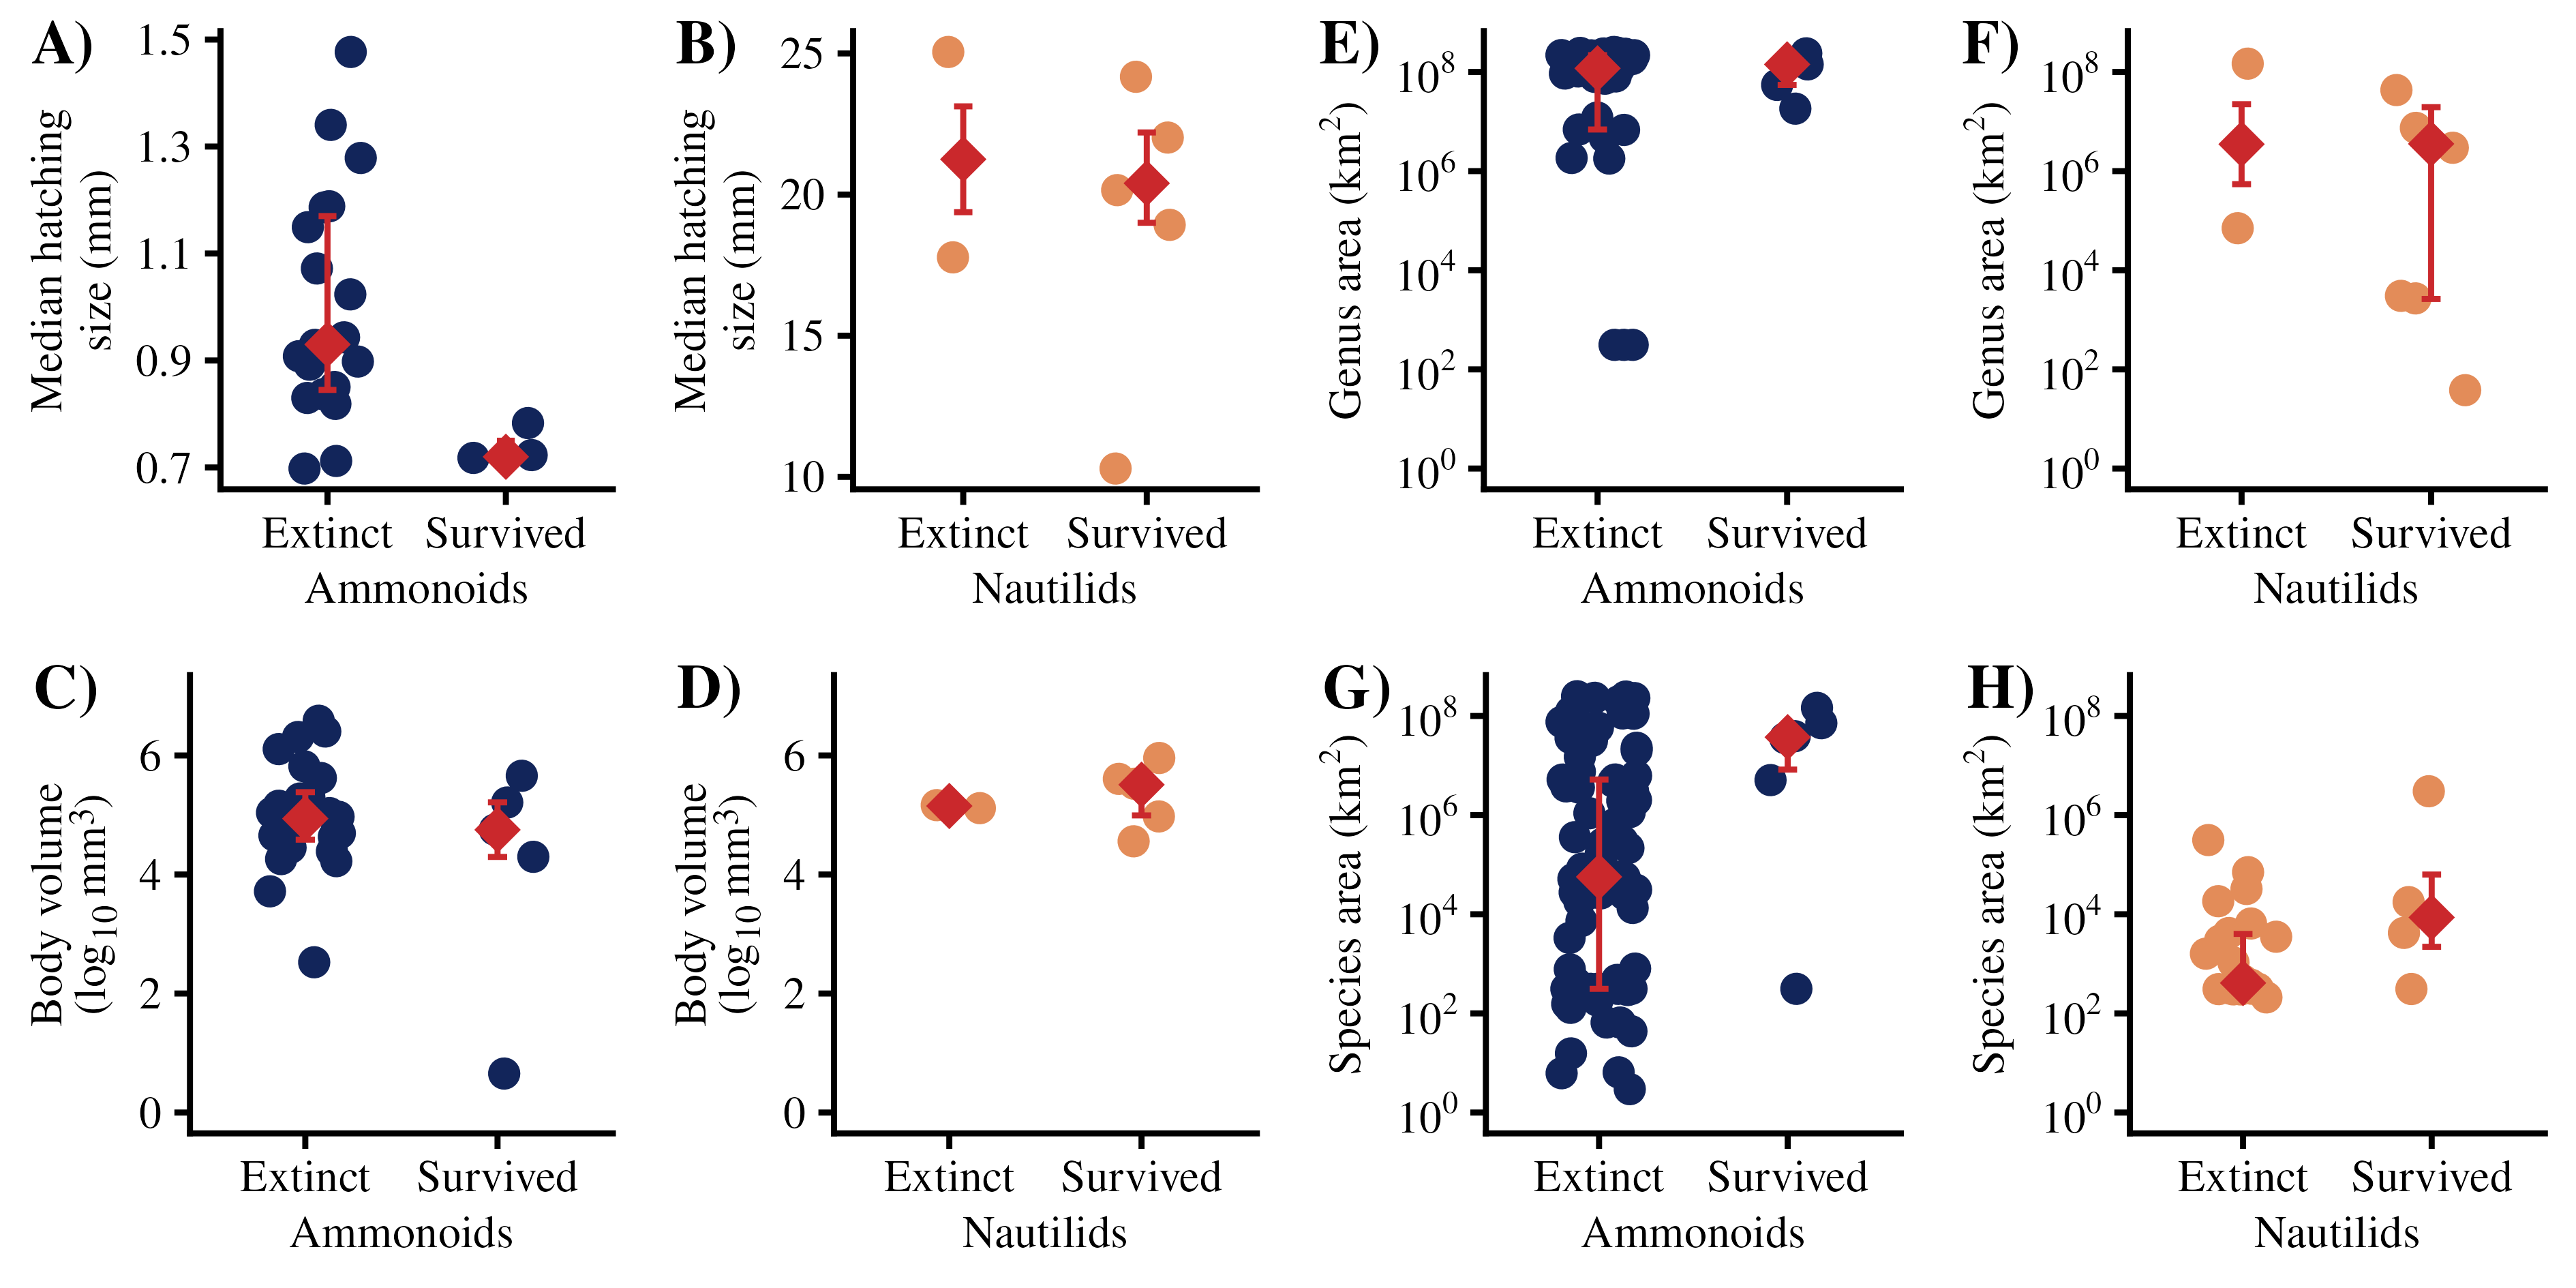
\includegraphics[width=\textwidth]{./figures/Data_figure.png}
\caption{Hatching size has the strongest association with short-term survival across the K-Pg of ammonoids. We assess three different predictor variables of survival at the genus level: Size at hatching of a) ammonoids and b) nautilids, adult body size of c) ammonoids and d) nautilids, and geographic range size of e) ammonoids and f) nautilids. We also consider geographic range sizes at the species level for g) ammonoids and h) nautilids. Hatching sizes are measured as the diameter of the shell at hatching (see for example \textcite{laptikhovskyEnvironmentalImpactEctocochleate2013}, other references in main text), and we report them as the median across species of a genus. 
Please note the difference in the vertical scales between a) and b). Other plots share the same scales for the same predictor variable. 
Body volume is estimated as the shell volume \parencite{payneBodySizeSampling2020, heimCopesRuleEvolution2015}. We estimate Maastrichtian geographic range based on fossil occurrences from the PaleoDB and \parencite{flannery-sutherlandLateCretaceousAmmonoids2024}. We reconstruct the palaeo-coordinates of these occurrences using plate tectonic models, and report the area of a minimum convex hull that encases their locations. 
We use several models (details in Methods section), but here we show geographic range based on the PALEOMAP plate tectonic reconstructions \parencite{scotesePALEOMAPPaleoAtlasGPlates2020}.
In all plots, red diamonds indicate the median, and the red error bars show the interquartile range.
}
\label{fig_data}
\end{figure}

%- Show and describe raw data. Point out strong difference between ammonoid survivors and extinct genera in median hatching size
% Maybe mention abundance as well. Put all that in supplement
%- Discuss sensitivity analysis. Bootstrapping. Jackknifing. Removing marine areas. In SUPPLEMENTARY MATERIALS
%- Describe weight of evidence argument. Draw on meta-analysis approach. Determine study power.
%- hatching size well supported and enough power for ammonoids
%- Describe how nautilids show no clear pattern, and that data is heavily underpowered

%We first describe what we observe in the data, and then infer in how far the associations we see between our predictor variables and survival have statistical support.

When we look at the data, the most striking difference we see is that ammonoid genera that survive in the short-term have among the smallest hatching sizes (figure \ref{fig_data}a). 
We note that all survivors belong to the ancycloceratina, which are characterised by small hatching sizes (SUPPLEMENTARY FIGURE).
Median nautilid genera do not appear to differ in hatching size, but there are few observations and considerable variation within and between genera (figure \ref{fig_data}b AND SUPPLEMENTARY FIGURE). % and within
Neither ammonoid nor nautilid adult body sizes (figure \ref{fig_data}c and d, respectively) show much difference between extinct and surviving genera. 

At the genus level, the geographic range sizes of surviving and extinct ammonoids do not differ substantially (figure \ref{fig_data}e). The same is the case for nautilids (figure \ref{fig_data}f), though again with few observations and a rather large variance. At the species level, we observe quite different patterns. Ammonoid species that survived the impact tend to have large geographic range sizes (figure \ref{fig_data}g). Though some extinct ammonoid species have similarly large geographic ranges, extinct ammonoids show considerable variation in range size. Consequently, the median geographic range size of extinct ammonoid species is almost three orders of magnitude smaller than that of surviving ammonoids ($5.68\times 10^{4}$ km$^{2}$ compared to $3.74\times 10^{7}$ km$^{2}$, respectively). For nautilid species, surviving species appear to have a larger median geographic range size, but the difference is small compared to the variation between genera (figure \ref{fig_data}h).

[DISCUSS SUBSAMPLING PROCEDURES AND DIFFERENT PLATE TECTONIC MODELS]

The low number of nautilid taxa and ammonoid survivors makes the statistical analysis of our data challenging. We therefore opt for a meta-analysis approach that allows us to weigh how well our data supports different hypotheses. We also assess whether our study has enough power to infer statistical associations between our predictor variables and survival \parencite{quintanaGuideCalculatingStudyLevel2023}.
We do not report effect sizes or power analyses for species-level subsampling for nautilids because only a single surviving species can be subsampled, which makes inferring confidence intervals and statistical power impossible. 

To begin, we report the differences between surviving and extinct taxa in terms of the common language effect size, a measure closely related to Mann-Whitney's $U$ \parencite{permeConfidenceIntervalsMann2019}. This effect size is an intuitive measure of the probability that an extinct taxon has a larger value of the predictor variable of interest than a surviving taxon. At an effect size of one, all extinct taxa have larger values than the surviving taxa, and the reverse is the case at an effect size of zero. If there are no true differences between extinct and surviving taxa then the expected effect size is 0.5, as by random chance half of the extinct taxa will have larger values. We reject the null hypothesis of no true difference if the confidence interval of the effect size does not include 0.5, with an $\alpha$ level of 0.05. 

%Sensitivity analysis: Run with all kinds of CI methods. 
The effect sizes for our predictor variables and several sensitivity analyses are shown in figure \ref{fig_power}a and b for ammonoids and nautilids, respectively. 
For ammonoids, the effect size measure supports the observation that surviving ammonoids had substantially smaller hatching sizes (effect size of 0.894 confidence interval 0.657-0.974). 
In line with our observations above (figure \ref{fig_data}c), we accept the null hypothesis of no difference in adult body size between surviving and extinct ammonoids.
When it comes to geographic range size, the evidence is less clear-cut. While the raw and subsampled data at the species level tend towards showing that survivors had larger geographic ranges sizes, this is only statistically supported when outliers are ignored (jackknife analysis). At the genus level, effect sizes are conflicting but tend to hover around the null expectation. 
For nautilids, confidence intervals are very wide, and the null hypothesis cannot be rejected for any predictor variable (figure \ref{fig_power}b). 

\begin{figure}
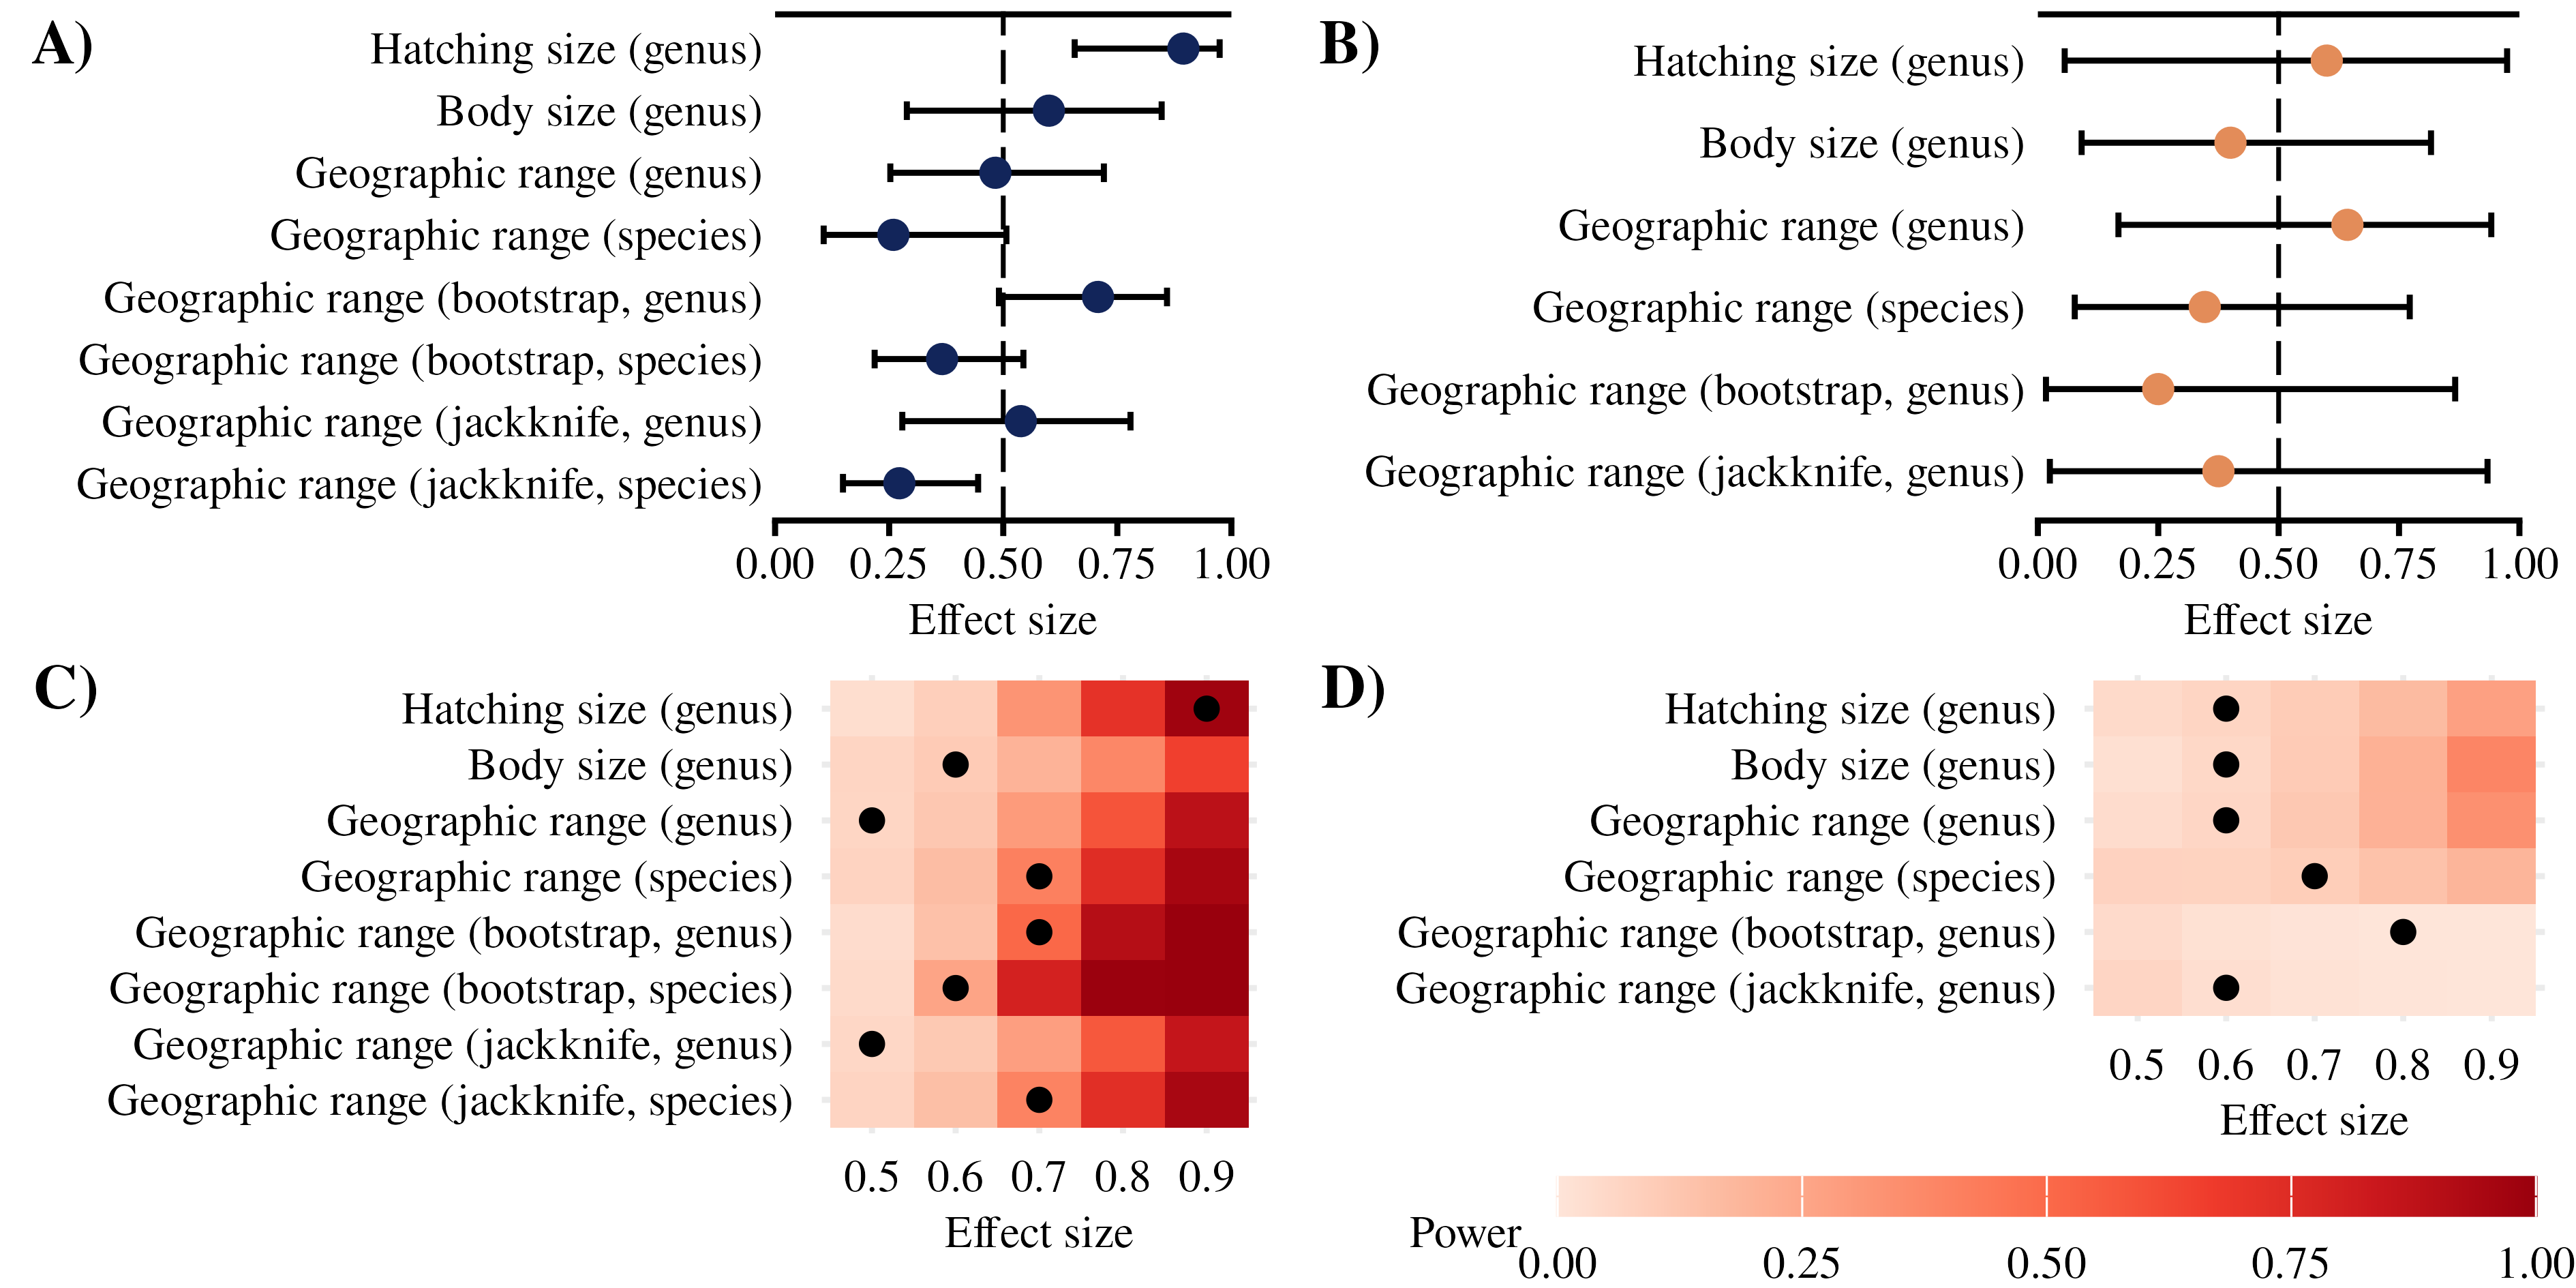
\includegraphics[width=\textwidth]{./figures/Effect_size_power_figure.png}
\caption{Common language effect sizes for our predictor variables and subsampling analyses (bootstrap, jackknife) for a) ammonoids and b) nautilids. 
Maximum effect sizes are zero or one. At an effect size of one, all extinct taxa have larger values than surviving taxa, and the opposite at an effect size of zero. An effect size of 0.5 is the null hypothesis (dashed line), which is rejected if the 95\% confidence interval does not intersect it. 
Statistical power of our study given the data available for our predictor variables, for c) ammonoids and b) nautilids.
We define power as the probability of recovering a true positive. 
We estimate power with simulated data that has the characteristics of our empirical data (relative variances and sample size), but different effect sizes. 
Black dots correspond to empirically observed effect sizes, rounded to the first significant figure, and flipped if it is less than 0.5 (i.e. an effect size of 0.3 is symmetrical to one of 0.7). 
Because subsampling analysis were possible for only a single surviving nautilid species, we did not calculate effect sizes or perform power analyses for subsampling analyses for nautilid species.
}
\label{fig_power}
\end{figure}


Next, we consider whether our study has sufficient power to detect a real effect given the data we have.
We estimate the power of our test using simulated data with the characteristics of our study data (relative variances and sample size) but different effect sizes (from 0.5 to 0.9). For ammonoids, statistical power is moderate  (0.5 or above) to good (0.8 or above) for effect sizes of 0.8 or 0.9 for all predictor variables (figure \ref{fig_power}c), with adult body size having the weakest power at an effect size of 0.9 (a power of 0.656).
For hatching sizes in ammonoids, the power at an effect size of 0.9 is 0.977, and thus our test has a good ability to discriminate the effect size we observe. 
However, our study is underpowered for all other predictor variables, with the second best power being a very moderate 0.508 at an effect size of 0.7, which corresponds roughly to what we see in bootstrapped geographic ranges at the genus level. This means that the probability of both false negatives and false positives is substantial for all other predictor variables at the effect sizes we observe. 

When it comes to nautilids, our study has almost no power. Even in the best case, adult body size and an effect size of 0.9, power does not exceed 0.388 (figure \ref{fig_power}d). This reinforces our observations when we considered the raw data (figure \ref{fig_data}) and the effect sizes (figure \ref{fig_power}b). Available nautilid data is insufficient to detect any signal.


\section*{Discussion}

In our study, we survey ammonoid and nautilid survival during the end-Cretaceous mass extinction. We examine three predictor variables with sufficient data at the genus level: Hatching size, adult body size, and geographic range size. The latter we also examine at the species level. We compare the predictive ability of these variables using meta-analytic techniques, and assess in how far the data we draw on in this study is sufficient to address our question.
We find that our data is informative for ammonoids only. We will therefore discuss ammonoid-specific results in the following paragraphs, before considering the issues that arise with nautilids. 

As far as ammonoids are concerned, representatives of five genera can with some confidence be said to have shortly survived the asteroid impact (table \ref{tab_surv}). These genera are: \textit{Baculites}, \textit{Discoscaphites}, \textit{Eubaculites}, \textit{Fresvillia}, and \textit{Hoploscaphites}. It is unlikely that this is an exhaustive list.
We report substantial sampling bias in both nautilid and ammonoid occurrences world-wide, which is a well-known problem in contemporary fossil databases \parencite{rajaColonialHistoryGlobal2022}.
Unsurprisingly, rare and difficult to identify ammonoid survivors are known exclusively from very well sampled regions in North America and Europe (figure \ref{fig_locdensity}). 
Possibly, this distribution of survivors could indicate that there was something special about the Tethys and the young Northern Atlantic ocean that made ammonoid survival more likely in these regions. 
Indeed, the Tethys region may have been a refugium for crustaceans during the end-Cretaceous mass extinction \parencite{schweitzerSelectiveExtinctionEndCretaceous2023}.
% See also Harries et al (1996) Models for biotic survival following mass extinction
However, we believe it is more parsimonious to explain this pattern as a result of collection bias. This option also opens up the exciting possibility that more sites world-wide contain yet-undiscovered ammonoid survivors, and that the current set is heavily skewing our perception of ammonoid survival.
The recent discovery that \textit{Fresvillia} survived reinforces our point. It shows that even in well-sampled locations such as Stevn Klint in Denmark surprising discoveries can still be made \parencite{machalskiAmmoniteSurvivalCretaceous2025}. What may lie in wait world-wide?

%Confirmed ammonite survivors are known exclusively from highly sampled regions of the world: North America and Europe. 
%Short-term survival of communities elsewhere?
%Or is ammonoid survival limited to the Tethys, and was there something unusual about the Tethys in the aftermath of the impact? 

Keeping this uncertainty in mind, our strongest result implies that ammonoids with smaller hatching sizes had better chances of surviving the immediate aftermath of the asteroid impact. 
If we take this result at face value, then it has interesting implications for the nautilid survival -- ammonoid extinction question. 
That hatching size might have played an important role in the differential survival of nautilids has been a popular hypothesis for some time \parencite{stilwellRecordsNautiloideaMollusca1996, waniLargeHatchlingSize2011, debaetsEarlyEvolutionaryTrends2012, laptikhovskyEnvironmentalImpactEctocochleate2013, tajikaOldNewPlankton2018, tajikaIntraInterspecificVariability2022}. Indeed, there is an eye-catching difference in hatching size between ammonoids and nautilids.  
Yet our results imply that selectivity at the end-Cretaceous was not simply a question of preferring larger eggs. One interpretation could be that there were multiple strategies for survival, a nautilid one with large hatching sizes, and an ammonoid one involving small hatching sizes. Indeed, the other cephalopod survivors, the squids and octopuses (coleoids), also have small hatching sizes \parencite{fuchsEvolutionReproductiveStrategies2020}.
Possibly though, hatching size is not the relevant factor at all, but instead happens to be correlated with the true cause of survival in ammonoids.

We note that among all ammonoids in our dataset, the heteromorphic Ancycloceratids such as \textit{Baculites} and \textit{Hoploscaphites} had the smallest hatching sizes. Therefore, our results may simply be picking up on the fact that all known survivors are Ancycloceratids. Only a more fine-grained analysis involving more measurements of heteromorph ammonoid hatching sizes can disentangle whether this pattern holds and, say, hatching size is also predictive of survival within Ancycloceratida. Thus, though hatching sizes is the strongest predictor of short-term survival in ammonoids, it is not necessarily the trait that end-Cretaceous mass extinction selectivity acted upon. 

We should also caution that, due to a lack of data, our result is based on the median hatching size of genera.
However, there can be substantial variation within an ammonoid genus. This issue can only be addressed with more measurements, for although  hatching size measurements are available for 41 percent of late Cretaceous ammonoid genera, this only covers 6 percent of pertinent ammonoid species.

Possibly a similar limitation applies to adult body sizes, though we lack the species-level data to corroborate that. The measurements we draw on were made for only a single species per genus \parencite{heimCopesRuleEvolution2015, payneBodySizeSampling2020}. Adult body size has been implicated in other studies of selectivity during the end-Cretaceous mass extinctions \parencite{yingDarknessBodySize2026, friedmanEcomorphologicalSelectivityMarine2009, longrichMassExtinctionLizards2012}, but does not appear to have been of much importance for ammonoids.



In contrast to the previous landmark study of ammonoid extinction \parencite{landmanAmmoniteExtinctionNautilid2014}, we find only limited evidence for geographic range size playing a role in ammonoid survival. We find that ammonoid species that survived had larger geographic range sizes than the majority of species that went extinct immediately. However, this result is not statistically significant unless geographic outliers are discounted from our geographic range reconstructions. 
Possibly this is a false negative arising from our study design. Our time binning is less strict as that of the \textcite{landmanAmmoniteExtinctionNautilid2014} study. If the geographic ranges of ammonoids shifted considerably during the Maastrichtian, then a coarser time binning might cause us to infer geographic ranges that are inflated relative to the geographic ranges these animals actually occupied at the time of the impact.
The same time-averaging effect could explain why we see little difference between the geographic range sizes of surviving and extinct genera. 


%Mechanism of extinction may differ from other events
%- evidence that end-Triassic associated with thinner shells in ammonoids \parencite{weberRelativeThicknessAmmonoid2022} 
%- simplification in brachiopods and foraminifera during end-Permian mass extinction \parencite{wangBrachiopodsForamsReduced2025}
%- consistent with ocean acidification (REFS)
%- End-Cretaceous is different. The surviving heteromorphs all have very complex sutures

We caution that both the low number of ammonoid short-term survivors and the limited data on nautilids makes statistical analysis challenging. 
We opt for a method that is intuitive, flexible, and designed to work with small samples \parencite{permeConfidenceIntervalsMann2019}. 
Still, to make this analysis work we assume exchangeability of data points. This assumption may not hold when traits are not independent due to common ancestry
\parencite{churchillNaiveApplicationPermutation2008, felsensteinPhylogeniesComparativeMethod1985}.

The greatest limitation of our study though is that nautilids suffer from relative neglect. Nautilid occurrences are rare \parencite{landmanAmmoniteExtinctionNautilid2014, stilwellRecordsNautiloideaMollusca1996}, their taxonomy understudied \parencite{lehmannOriginEvolutionaryHistory2017, wardNautilusBiologySystematics2016, wilmsenLateCampanianNautiloids2019, chiratShellMicrostructureMorphogenesis2006}, and their survival across the K-Pg boundary poorly understood (this study). Our power analysis shows clearly that, for the predictor variables we examine, there are too few nautilid taxa and too much variation between nautilids to make any inference. Possibly, extinction selectivity in nautilids depended upon factors we have not examined, or was in fact random. Most likely though nautilids are too little studied and their taxonomic affinities muddled. 
We will not understand nautilid survival and their persistence to the present day unless we improve their taxonomy and study their traits and ecologies with greater care. If we do, they may yet leave us with lessons in tenacity invaluable in our current-day biodiversity crisis.


In sum, based on this study we recommend the following research focuses to better understand ammonoid extinction and nautilid survival:
\begin{itemize}
\item Revise nautilid taxonomy
\item Search for nautilids around the K-Pg boundary
\item Measure hatching sizes in more Cretaceous ammonoids, especially heteromorphs
\item Search for ammonoid survivors globally.
\end{itemize}

However, these are not the only promising avenues for future research. Other factors should be explored too, for example differences in ammonoid and nautilid metabolic rates \parencite{tajikaAmmonoidExtinctionNautiloid2023}, or in their ecologies (which could be inferred from the depositional environment), and changes in biological interactions \parencite{garcia-gironShiftsFoodWebs2022}. 
There has also been, to our knowledge, no attempt to measure calcification costs of late Cretaceous ammonoids or nautilids, as has been done for ammonoids that experienced the end-Triassic mass extinction \parencite{weberRelativeThicknessAmmonoid2022}. Such measurements might shed light on the role of ocean acidification during the end-Cretaceous, which is contentious \parencite{yingDarknessBodySize2026, henehanRapidOceanAcidification2019}.
%Something general about mass extinctions?


Future studies should also focus on the other group of cephalopods that survived: The coleoids. Coleoids are the closest living relatives of ammonoids. Because the largely soft-bodied coleoids do not fossilise well \parencite{krogerCephalopodOriginEvolution2011}, little is known about their survival at the end-Cretaceous mass extinction. However, new advances in grinding tomography coupled with machine learning \parencite{ikegamiOriginRadiationSquids2025, ikegamiSquidsRadiatedGlobally2026} has lead to the discovery of fossilised cephalopod beaks that could not be recovered previously, exposing rich Cretaceous coleoid communities. 
In the coming years, these advances should allow more thorough quantification of cephalopod diversity change during the end-Cretaceous mass extinction, filling in an important gap in our understanding of cephalopod evolution and extinction resilience.  

\printbibliography

\end{document}